\section{Results}
\label{sec:results}

%All the experiments were performed on the Blue Gene/L supercomputer. 

\begin{figure}
\begin{center}
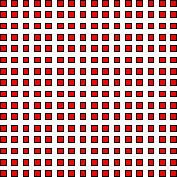
\includegraphics[keepaspectratio]{full_16_16}
  \caption{Full distribution. Each red square represents a processor with data}
  \label{fig:full_4096}
\end{center}
\end{figure}

\begin{figure}
\begin{center}  
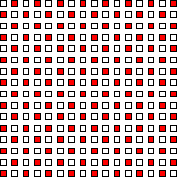
\includegraphics[keepaspectratio]{checkerboard_16_16}
  \caption{Compressed Checkerboard Distribution. Each red square represents a processor with data while a white square represents a processor without any data}
  \label{fig:checkerboard_4096}
\end{center}
\end{figure}

\begin{figure}
\begin{center}
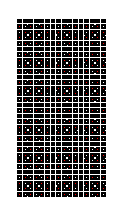
\includegraphics[keepaspectratio, , height=2.8in]{checkerboard_16_32}
\end{center}
\caption{Expanded Checkerboard Distribution.Each red square represents a processor with data while a white square represents a processor without any data}
\label{fig:checkerboard_8192}
\end{figure}

In this section we explore the effects of mapping on the performance
of the transpose operation on BG/L. Because the transpose required by
the BGL3DFFT algorithm uses three \alltoall communication
operations, the first along independent node columns and the rest
along independent node planes, the results presented below are for
columnar and planar \alltoall collectives implemented with both the
MPI and SPI communication layers. Because of the lower overhead
incurred by the SPI implementation, the effects of mapping are more
pronounced in that case and our discussion of results focuses on the SPI
implementation. The motivation is two fold: i) to evaluate the cost of individual transpose operations 
using three different data distributions; and ii) show that
the expanded checkerboard distribution slightly improves 3D-FFT performance and thus 
extends the scalability of Blue Matter on BG/L.

\subsection{Distributed Transpose performance}
\label{sec:transpose}

Consider performing a $64^3$ complex to complex (double precision)
3D-FFT on two different partition sizes, $16 \times 32 \times 16$ and
$16 \times 16 \times 16$ nodes where both use only half of the
available nodes in each partition for 1D-FFT computation.  The nodes
used for 1D-FFT computation in each partition form a checkerboard
pattern. We refer to them as the ``expanded checkerboard distribution''
the ``compressed checkerboard distribution'' respectively.  The
data is initially distributed equally to all nodes, each of
which holds, $n_x\times n_y\times n_z$ complex double data, where
$n_i=\frac{N_i}{P_i}$ and $i$ denotes $x,y$ or $z$.
 
Figures~\ref{fig:checkerboard_4096} and \ref{fig:checkerboard_8192}
illustrate the data distributions (in a single plane) of each
communication phase for both ``checkerboard'' distributions. 
Figure~\ref{fig:full_4096} shows the corresponding data distributions
for computing the 3D-FFT using all 4096 nodes, the ``full
distribution'', for comparison.

Tables~\ref{tab:a2a_z}, \ref{tab:a2a_y} and \ref{tab:a2a_x} show the
performance data for the full and both checkerboard distributions.
Column one describes the data decomposition and the number of nodes
performing the 3D-FFT out of the total available nodes in the machine.
For example, checkerboard (4096/8192) means that originally, the data
is distributed on 8192 nodes while the 3D-FFT is computed on 4096
nodes. Columns 4 and 5 contain the total elapsed time per
communication phase for the corresponding data distributions.  In all
the performance tables, we provide the results in terms of average elapsed
time over 100 runs (omitting the first run).  The error bars signify the standard deviation
from the average value.

Columns 4 and 5 in Tables ~\ref{tab:a2a_z}, ~\ref{tab:a2a_y}, and
~\ref{tab:a2a_x} compare the distributed transpose performance in all
3D-FFT communication phases on both the MPI and SPI-based
implementations.  In general, all the MPI and SPI results are
consistent in the sense that they exhibit similar relative performance
behavior for a given case.  We observe that the SPI-based \alltoall
implementation is about 2 to 4 times faster than the MPI-based
implementation for very small size messages. For small messages the
software overhead associated with sending a packet in the MPI-based
implementation is larger than the SPI. For example, in the expanded
checkerboard distribution each node sends data comprising a complex double
(32~bytes) in the planar transpose.  We note that 32~bytes data fit in
a single SPI packet while in the MPI-based approach
the messages are double the size ($64$~bytes, MPI has 3~quads of protocol, $48$~bytes). % Double check this
Thus, the SPI approach is superior at the limits of scalability.

Table ~\ref{tab:a2a_z} shows the performance of the \alltoall operation
along the $z$~column nodes and Figure~\ref{fig:comm_z} the $z$~plane of all
studied decompositions. Let's compare the compressed checkerboard
decomposition with the full decomposition using the SPI results.
Since all the 1D-FFTs along the $z$~dimension are independent we need
only consider the case of a one-dimensional grid of the $P_z$ nodes
that compute $n_x \times n_y = 16$ one-dimensional FFTs of size $64$.
In both distributions, the number of nodes along the z axis is the
same, $P_z$. In the full distribution every node exchanges data with
all the nodes in the same column, while in the checkerboard
distribution each node sends data only to half of the nodes in the
column. For instance, in the full distributions, each node in a column
in the torus sends packets of data length of 110~bytes. That is, 
a 64~byte payload (4 complex doubles) will fit into a bytes packet. Each packet also
has a 4~ byte CRC appended to it and results in an 8~byte acknowledgment; in addition
there are typically 2~bytes of unused space in each packet. Thus a
single 64~byte packet results in a 100~byte load on the link with a
packet utilization of $64/110 = 58\%$.
% This packet length, includes 14~bytes for packet header and payload of size of 4
%complex double ($4 \times 16$~bytes). 


%each node along a given
%z axis sends a message of a total length
% $((4* complex <doubles> )*\frac{8bytes}{double}+32) + (4+8+2)$
% bytes packet header $96+14=110$, to every node along the same axis, with packet
%utilization $\frac{64}{110} \time 100 = 58 \%$. 

In the checkerboard  distribution, there are 16 sender nodes, each sending 8 complex doubles 
to 8 destination nodes along a column of nodes in the torus.
That is, each nodes in the checkerboard distribution sends a packet of size $174~$bytes to 
alternate nodes, with packet utilization $128/174 = 73\% $.
 
%  Each processor in the checkerboard
%distribution sends a packet of size $160+4+8+2 = 174$ bytes (16
%complex doubles) to alternate processors, with packet utilization
%$\frac{128}{174} \times 100 = 73 \% $.

The average number of hops is 4, the same for both distributions, 
%need to double check this with Philip
%(${0+1+2+3+4+5+6+7+8}\{9}$) and (${0+1+2+3+4+5+6+7+8/2}{9})$ 
%for the full and  checkerboard,respectively, 
using the torus network.  Overall we observe efficiency
$29.58/35.841=0.82$ for the communication cost along a given column in
the compressed checkerboard distribution, which is consistent with the
prediction of $58\%/73\% = 0.79$.
 
Now, let's compare the full distribution to the expanded checkerboard
processor mesh.  Every processor along a column of nodes has 
to compute $16$ 1D-FFTs in the full distribution and $8$ 1D-FFTs 
%128bytes and 64bytes of data to send in the same number of nodes, 
in the expanded checkerboard distribution.  In both, each node sends
messages of the same length, $110$~bytes. However, in the checkerboard
distribution the bandwidth required is halved since each node sends
half as many packets.  The ratio of the measured communication
times is $35.841/19.944 = 1.90$ very close to the factor of two
predicted from bandwidth considerations.


\newcommand{\goodgap}{%
\hspace{\subfigtoskip}%
\hspace{\subfigbottomskip}}

\begin{figure}
\subfigure[Full distribution on $z$ column of processors. Each column of processor along the z axis computes 16 1D-FFTs of size 64, with each processor computing one 1D FFT. In the communication phase, all nodes of the left blue column sends data to the nodes of the column on the right of the arrow. 
%That is, each node on the left column sends data of size 4 complex doubles to all 16 processors on the right column. Each node on the right column receives data of size 4 complex doubles from all 16 processors on the left column.
]
{
  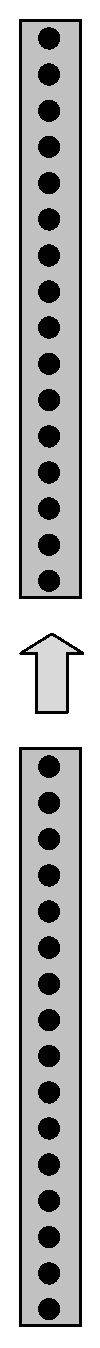
\includegraphics[keepaspectratio, angle=270,  width=3.1in,]{full_z}
  \label{fig:full.z}
} \\
\subfigure[Compressed checkerboard distribution on the $z$ column of processors. Each column of processor along the z axis computes 16 1D-FFTs of size 64, with each alternative processor computing two 1D FFTs. In the communication phase, all nodes of the left blue column sends data to half of the nodes(filled circles) of the column on the right of the arrow. 
% That is, each node sends data of size 8 complex doubles to 8 processors. Each alternative node (filled circles) on the right column receives data of size 8 complex doubles from all 16 processors on the left column.
]
{
  \includegraphics[keepaspectratio, angle=270,  width=3.1in]{comp_z}
\label{fig:comp.z}
} \\
\subfigure[Expanded Checkerboard on $z$ column of processors. Each column of processor along the z axis computes 8 1D-FFTs of size 64, with each alternative processor computing one 1D FFTs. In the communication phase, all nodes of the left blue column sends data to half of the nodes(filled circles) of the column on the right of the arrow. 
%That is, each node sends data of size 4 complex doubles to 8 processors. Each alternative node (filled circles) on the right column receives data of size 4 complex doubles from all 16 processors on the left.
]
{
  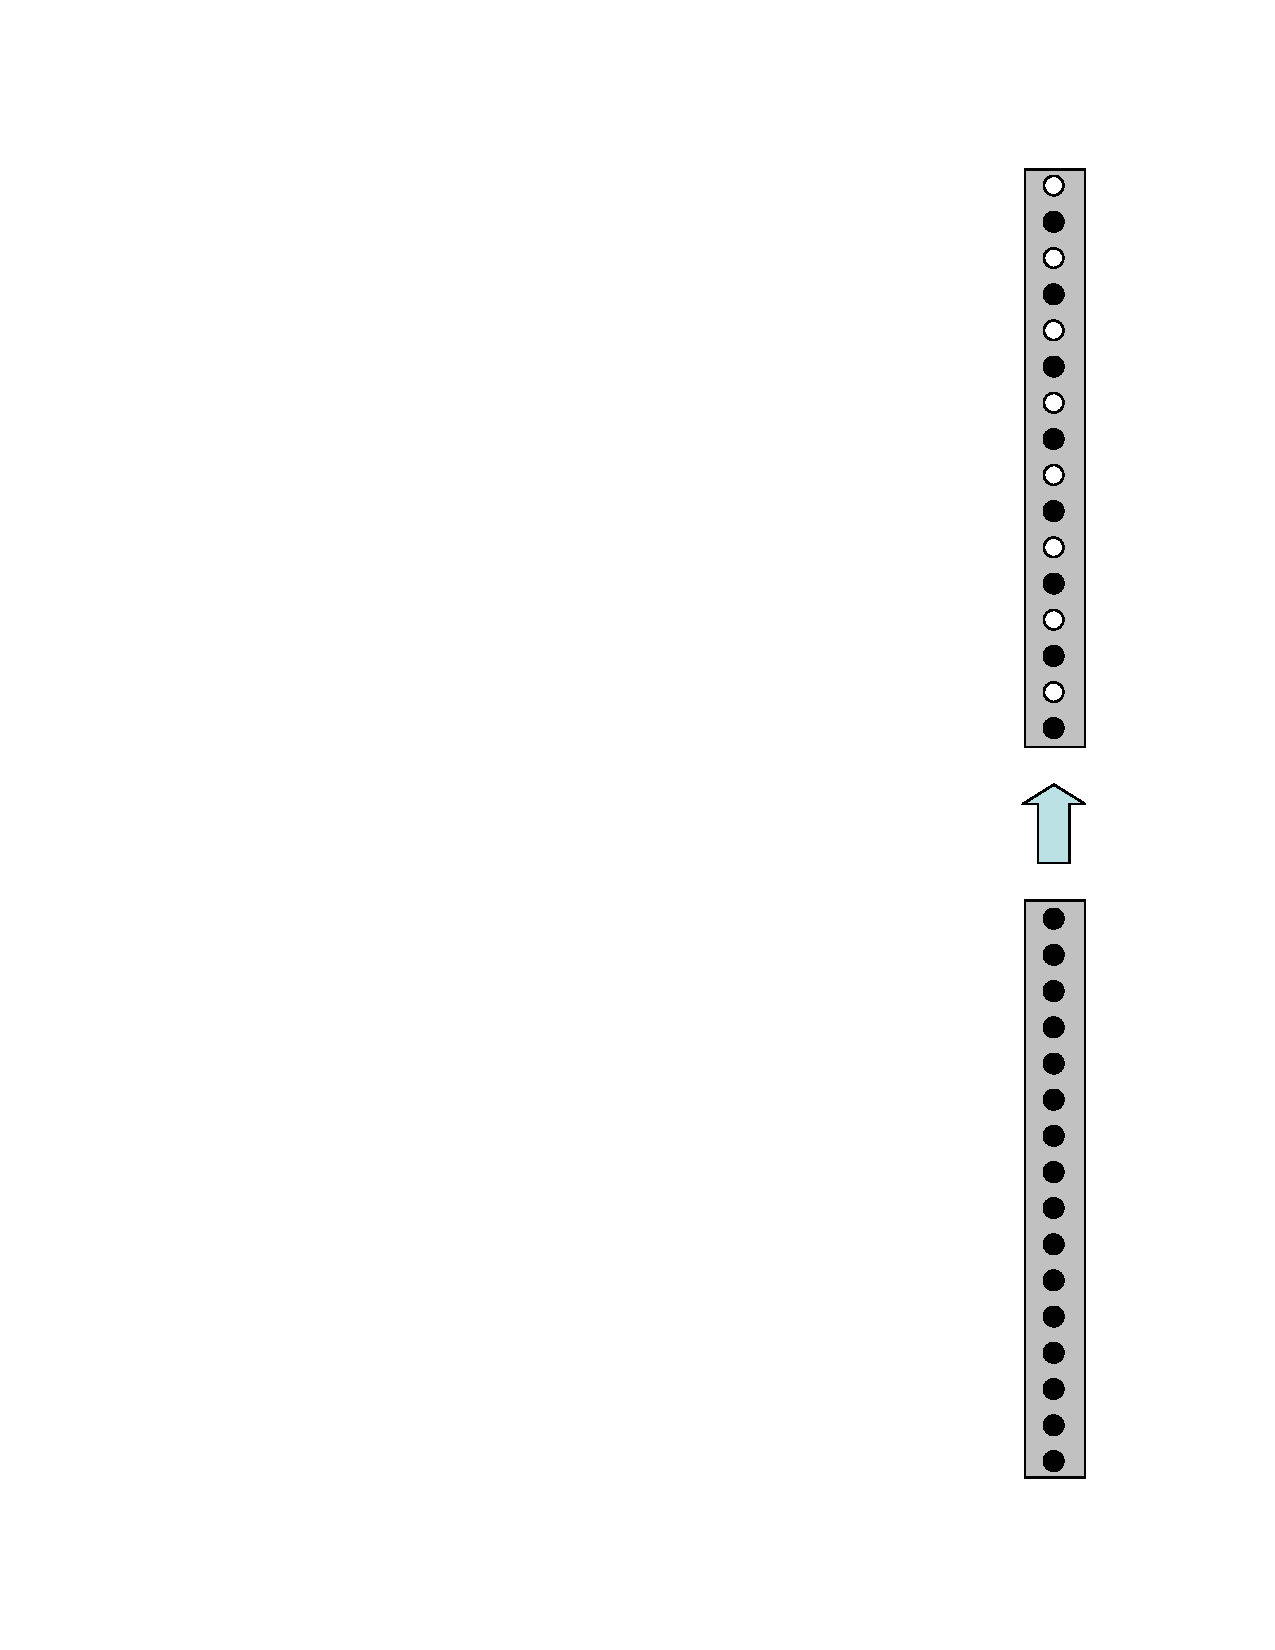
\includegraphics[keepaspectratio, angle=270,width=3.1in]{expand_z}
  \label{fig:expand.z}
}\\
\caption{Data distributions along the $z$ processor column. The filled circles represent nodes with data, while the empty represent nodes without any data.  On the compute phase, each column of processors along the z axis computes $n_x \times n_y = N_x/P_x \times N_y/P_y$ 1D-FFTs of size $Nz$, with each processor computing $(n_x \times n_y)/P_z$ 1D FFTs with $n_i=N_i/P_i$. }
\label{fig:comm_z}
\end{figure}

\begin{figure}
\subfigure[Full $zy$ plane of  $16 \times 16$ processors. Each $zy$ plane computes 256 1D-FFTs of size 64, with each processor computing one 1D FFT. In the communication phase, all 256 nodes of the left rectangle sends data to 64 nodes of the right of the arrow. 
%That is, each node of the blue rectangle sends data of size 1 complex doubles to all 64 processors on the right blue rectangle, etc. Each node on the right rectangle receives data of size 1 complex doubles from 64 processors of the left rectangle.
]
{
  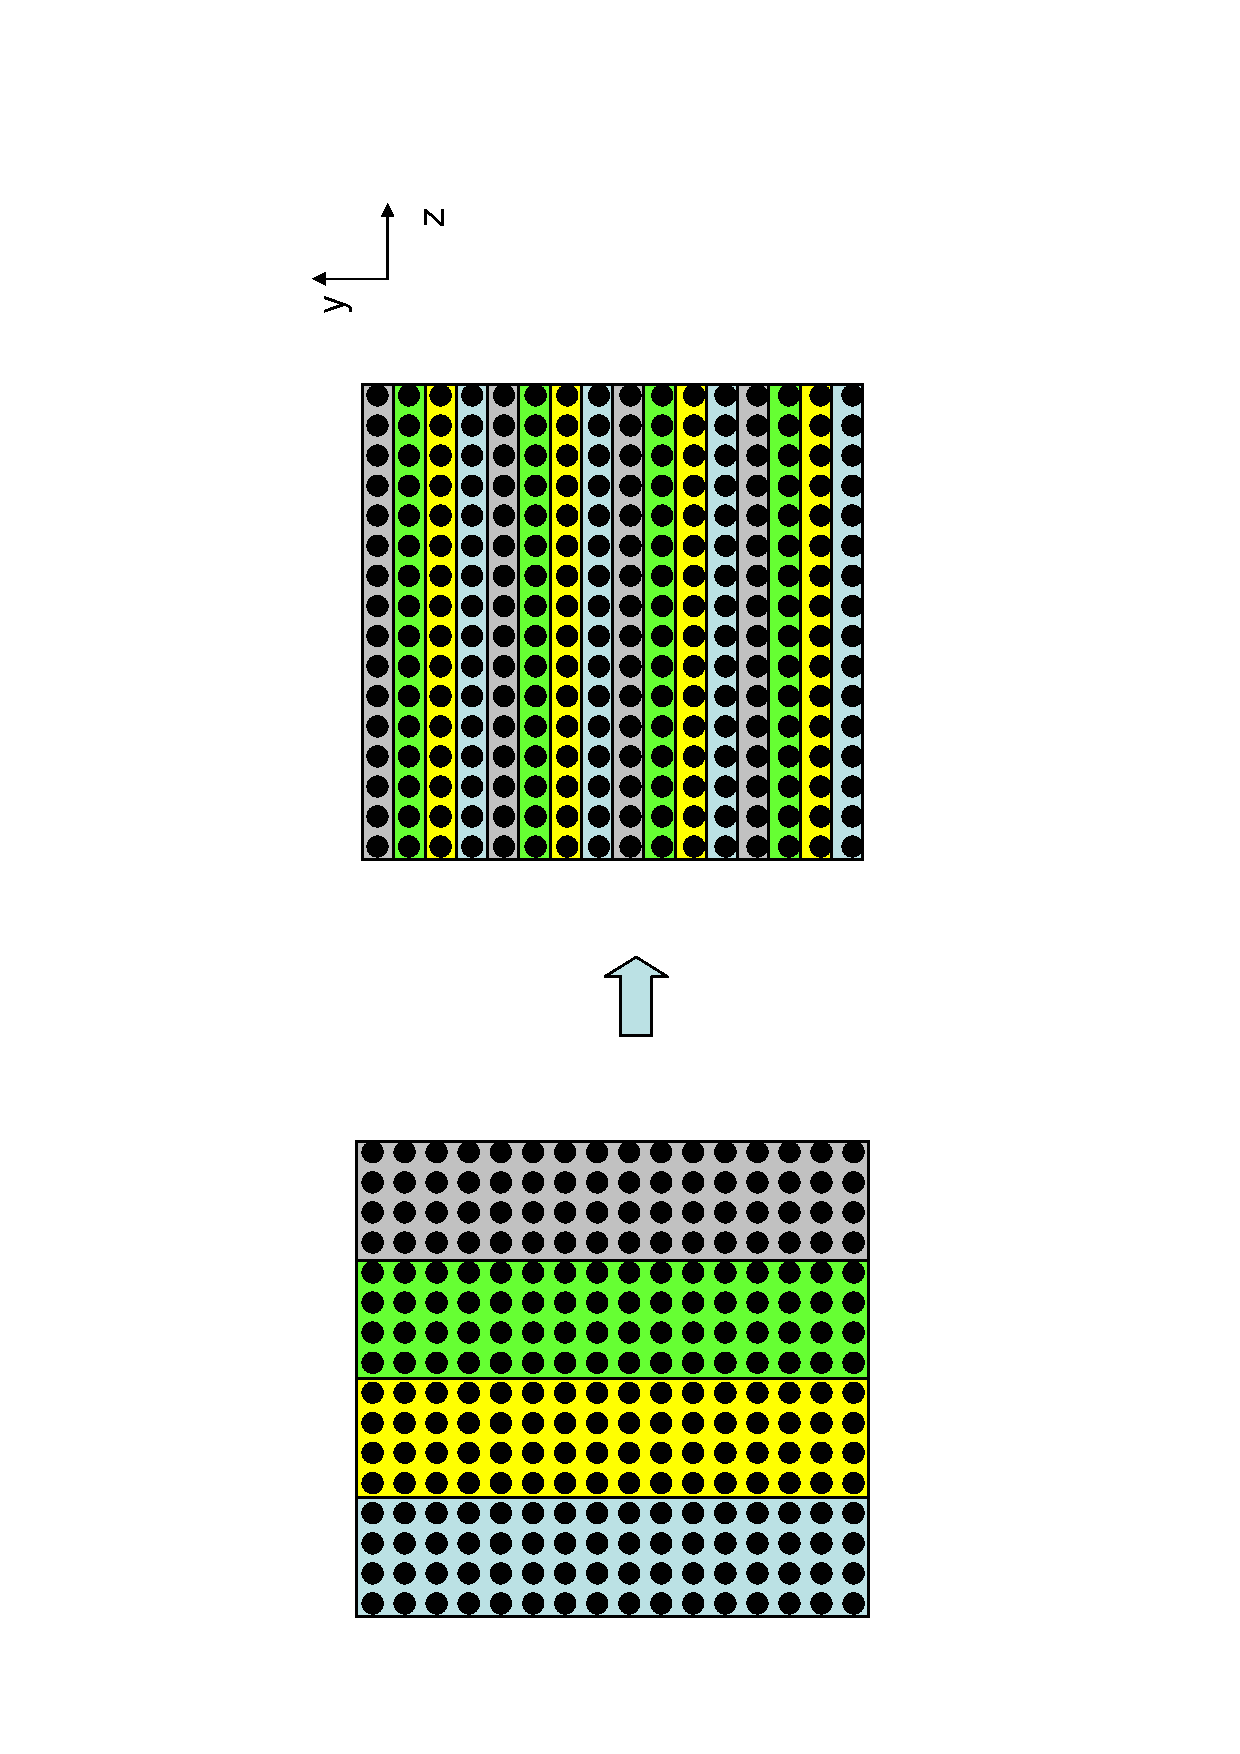
\includegraphics[keepaspectratio, angle=270,  width=3.1in]{full_zy}
  \label{fig:full.zy}
} \\
\subfigure[Compressed checkerboard $zy$ plane of $16\times 16$ processors. Each $zy$ plane of processors computes 256 1D-FFTs of size 64, with each processor computing two 1D FFT. In the communication phase, all 128 nodes (filled circles) of the left rectangle send data to 64 nodes of the rectangle on the right of the arrow. 
%That is, each alternative node of the blue rectangle sends data of size 2 complex doubles to all 64 processors on the right blue rectangles, etc. Each alternative node on the blue right rectangles receives data of size 2 complex doubles from 64 processors (filled circles) of the left blue rectangle.
]
{
  \includegraphics[keepaspectratio, angle=270,  width=3.1in]{comp_zy}
  \label{fig:comp.zy}
}\\
\subfigure[Expanded checkerboard $zy$ plane of $16\times 32$ processors. Each $zy$ plane of processors computes 256 1D-FFTs of size 64 along the $y$ dimension, with each processor computing one 1D FFT. In the communication phase, all 256 nodes(filled circles) of the left rectangle send data to  64 nodes(filled circles) of the rectangles on the right of the arrow. %That is, each alternative node of the blue rectangle sends data of size 1 complex doubles to all 64 processors on the right blue rectangles. Each alternative (filled circles) node on the blue right rectangles receives data of size 1 complex doubles from 64 processors(filled circles) of the left blue rectangle.
]
{
  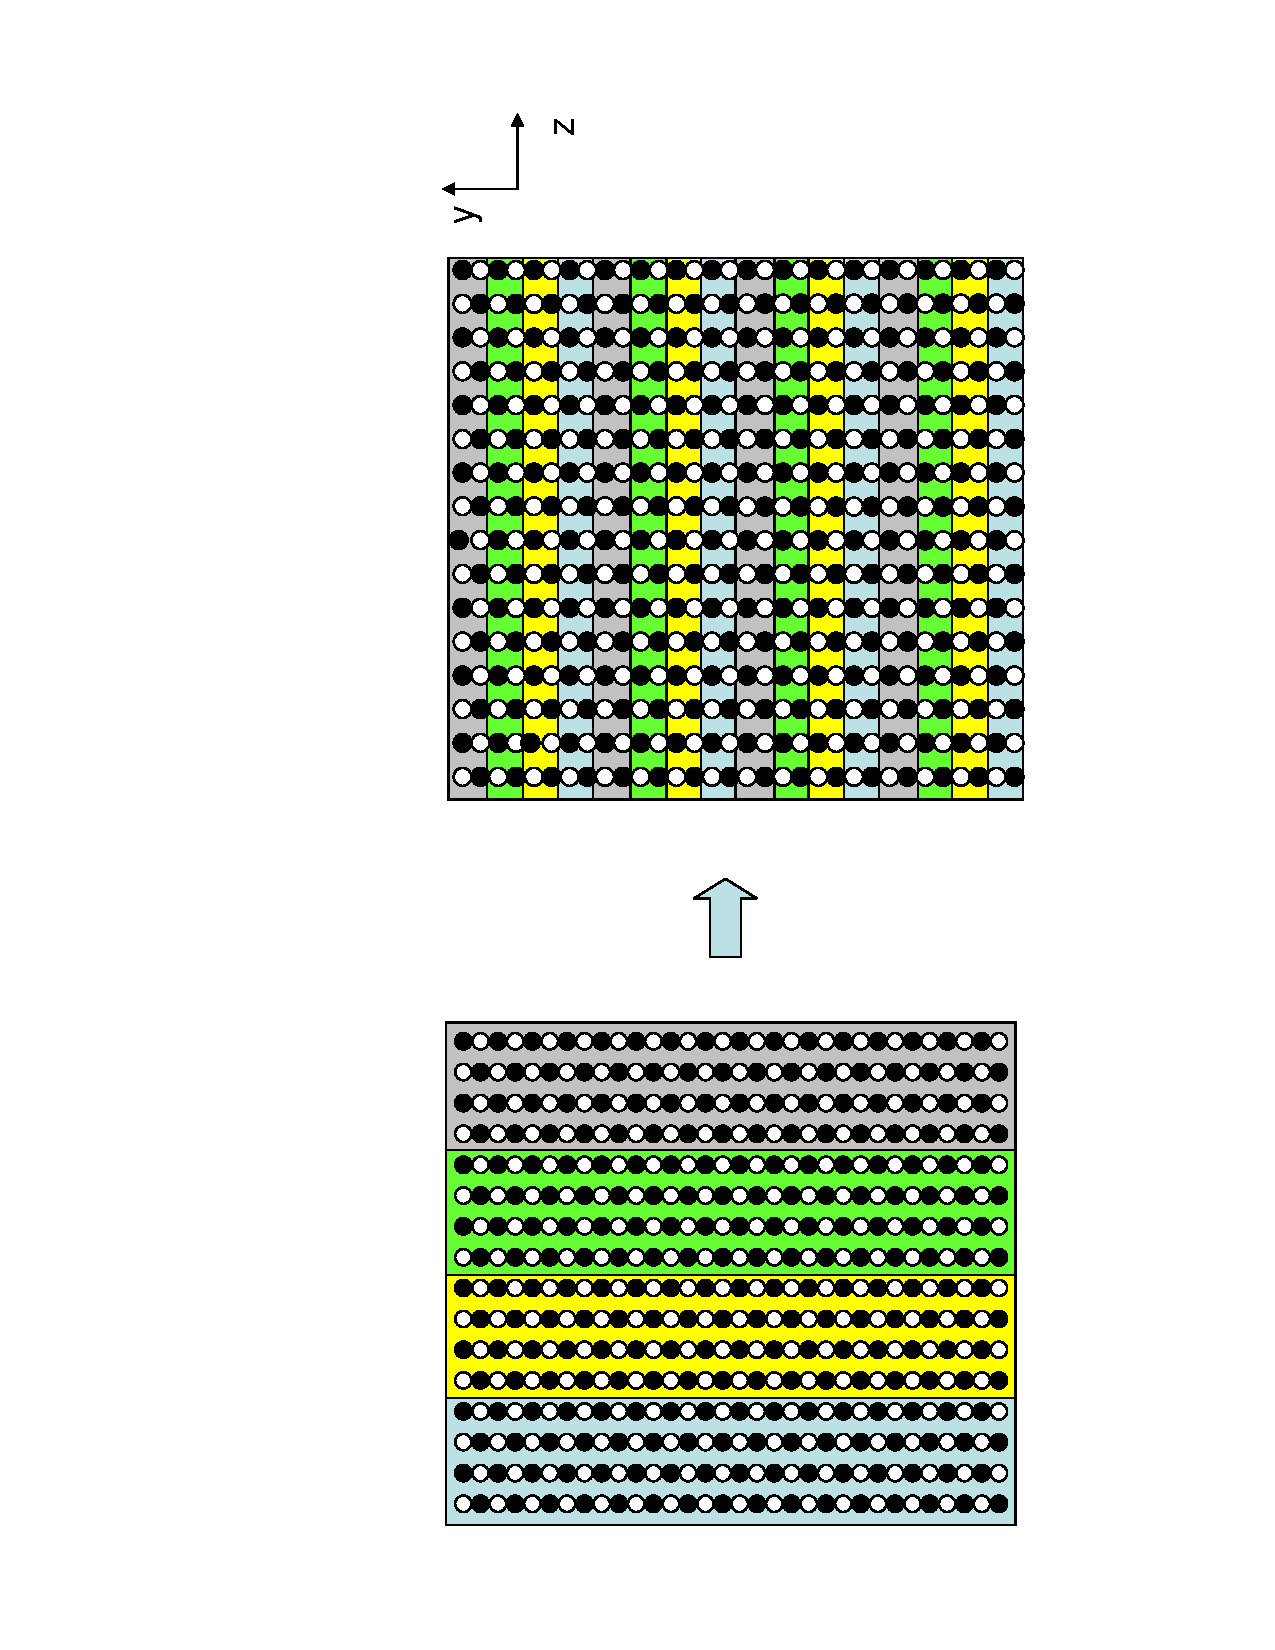
\includegraphics[keepaspectratio, angle=270,width=3.1in]{expand_zy}
  \label{fig:expand.zy}
}\\
\caption{Data distributions along the $zy$ processor plane of size $P_z \times P_y$. The filled circle represent nodes with data, while the empty represent nodes without any data. On the compute phase, each $zy$ plane of processors computes $n_x \times N_z $ 1D-FFTs of size $Ny$, with $n_i=N_i/P_i$. }
\label{fig:comm_zy}
\end{figure}

\begin{figure}
\subfigure[Full $yx$ plane of $16\times16$ processors. Each $yx$ plane of processors computes 256 1D-FFTs of size 64, with each processor computing one 1D FFT. In the communication phase, all 256 nodes of the left rectangle send data to 64 nodes of the rectangle on the right of the arrow. 
%That is, each node of the blue rectangle sends data of size 1 complex doubles to all 64 processors on the right blue rectangles. Each node on the blue right rectangles receives data of size 1 complex doubles from all 64 processors of the left blue rectangle.
]                                
{
  \includegraphics[keepaspectratio, angle=270,  width=3.1in]{full_yx}
  \label{fig:full.yx}
} \\
\subfigure[Compressed checkerboard $yx$ plane of $16 \times 16$. Each $yx$ plane of processors computes 256 1D-FFTs of size 64, with each processor computing one 1D FFT. In the communication phase, 128 alternative nodes(filled circles) of the left  rectangle send data to the 32 nodes of the rectangle on the right of the arrow. 
%That is, each alternative processor (filled circles) of the left blue rectangle sends data of size 4 complex doubles to 32 processors on the right blue rectangle. Each node on the blue right rectangle receives data of size 4 complex doubles from 32 alternative processors(filled circles) of the left blue rectangle.
]
{
  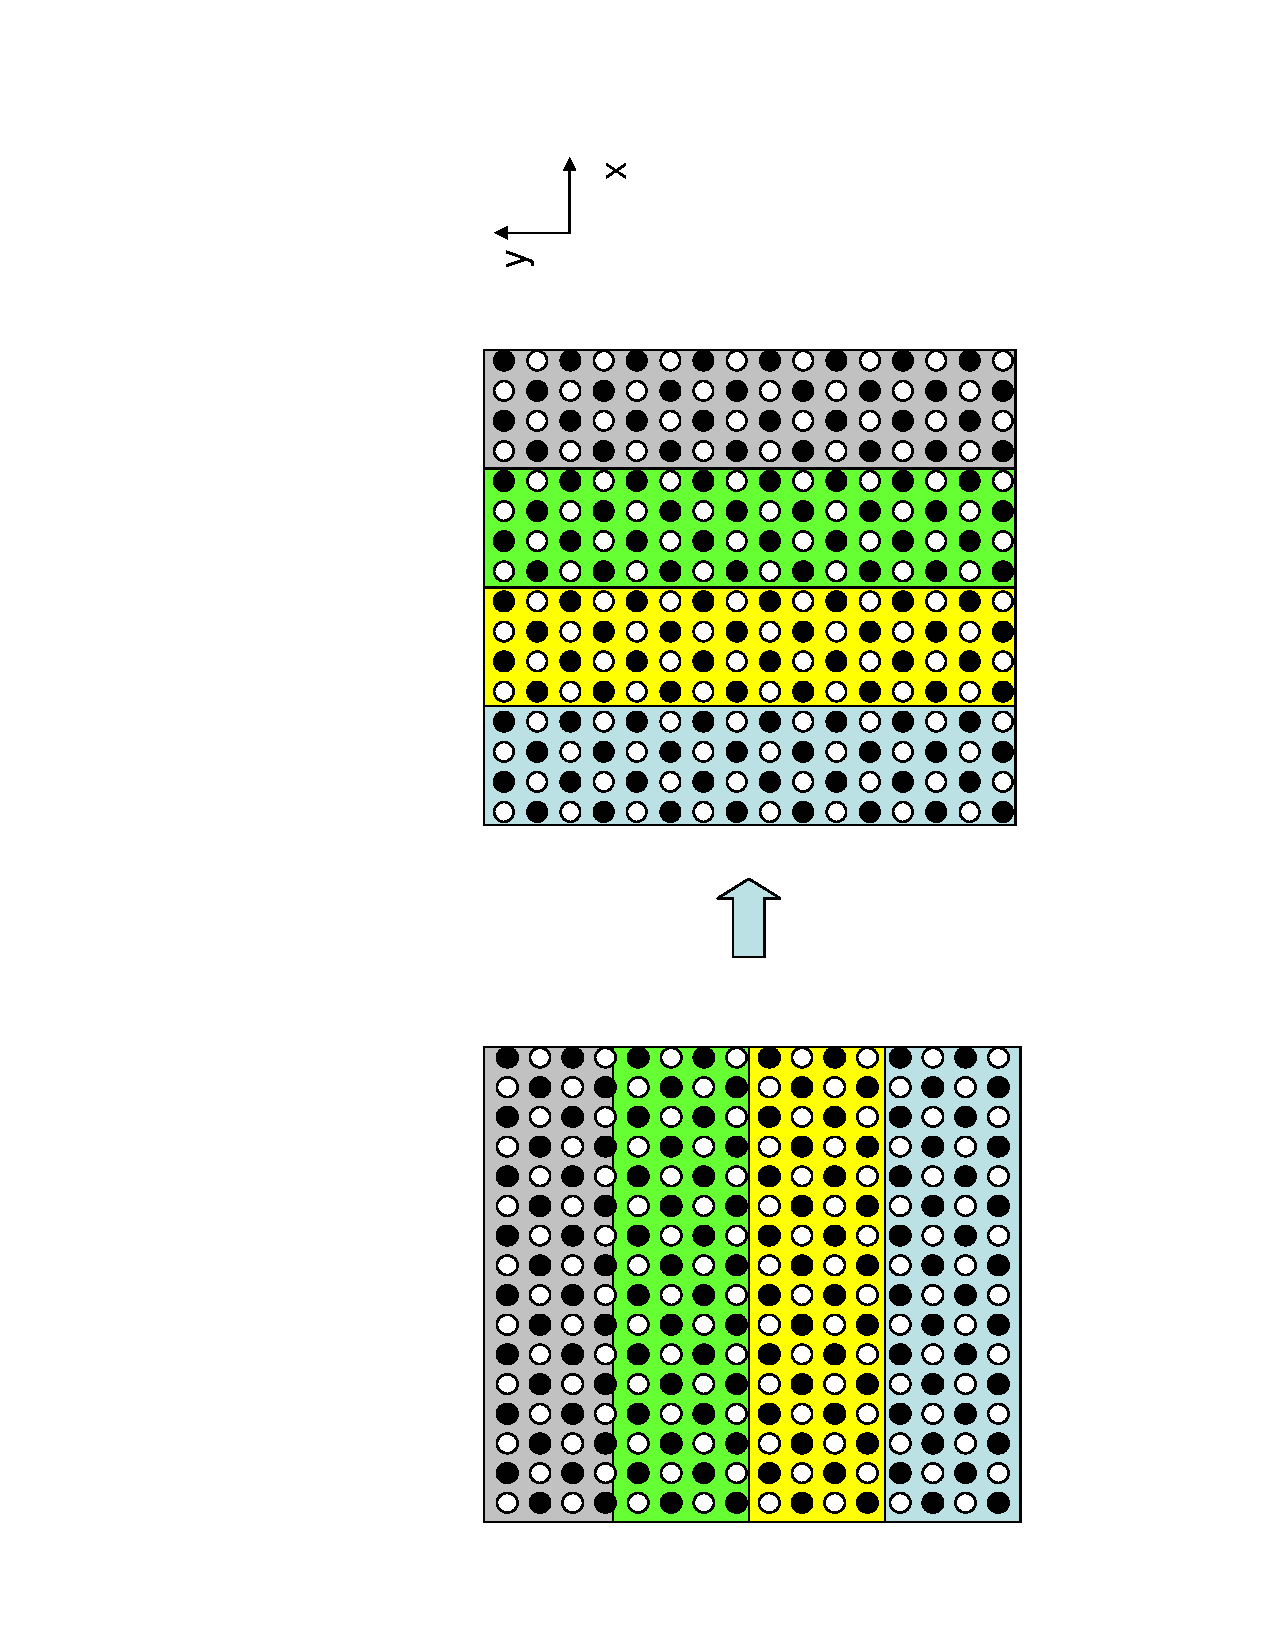
\includegraphics[keepaspectratio, angle=270,  width=3.1in]{comp_yx}
  \label{fig:comp.yx}
} \\
\subfigure[Expanded checkerboard $yx$ plane of $32\times 16$ processors. Each $yx$ plane of processors computes 256 1D-FFTs of size 64 along the $y$ dimension, with each processor computing one 1D FFT. In the communication phase, all 256 nodes(filled circles) of the left rectangles send data to  64 nodes(filled circles) of the rectangles on the right of the arrow. %That is, each node of the blue rectangle sends data of size 1 complex doubles to all 64 processors on the right blue rectangle. Each node on the blue right rectangle receives data of size 1 complex doubles from alternative 64 processors (filled circles) of the left blue rectangle.
]
{
  \includegraphics[keepaspectratio, angle=270,width=3.1in]{expand_yx}
  \label{fig:expand.yx}
}\\
\caption{Data distributions along the $yx$ processor plane. The filled circle represent nodes with data, while the empty represent nodes without any data. On the compute phase, each $yx$ plane of processors computes $N_y \times n_z $ 1D-FFTs of size $Nx$,  with $n_i=N_i/P_i$.}
\label{fig:comp_yx}
\end{figure}

Table ~\ref{tab:a2a_y} presents the \alltoall communication cost in the
$zy$-plane. For clarity, Figure~\ref{fig:comm_zy} shows only the data
distribution along a single plane $zy$ of nodes for all studied
distributions.  Let's first compare the performance of \alltoall in the
full and compressed checkerboard distribution.

% Send email to Chris to find out how many packets we send in the SPI for 2doubles.
In the full distribution, all nodes (256 total) exchange messages
of containing a single complex double with 64 nodes (including itself) in the
 plane, with packet utilization of $32/32=1$.   
%$\frac{32}{46}=0.69$.
In the compressed distribution, half of the nodes (128 total)
%$64+4+8+2=78$
exchange data with a packet size of $78$~bytes (2 complex doubles) with $64$ nodes
in a plane of nodes, with packet utilization $64/78=0.82$. 
Thus, we expect  $(32 \times 256)/(78 \times 128)=0.85$  
%$\frac{46 bytes \times 256nodes}{78bytes \times 128 nodes}=0.85$ 
which is consistent with the ratio of measured times, $55.305/58.131=0.95$
 
Next, consider the performance of the expanded checkerboard
$(4096/8192)$ distribution versus that of the full distribution
$(4096/4096)$. In the expanded checkerboard decomposition the
communication is performed on alternate nodes.  That is, half of
the nodes, $256$ out of $512$ don't exchange any messages. Each of the 
remaining  $256$ nodes sends packets containing one complex double to
$64$ (including self) destination nodes. 
% The number of nodes in y is double, implies the latency is double.. NEED to double check
%Thus each  message is of length $46$bytes ($1$ complex double). 
Similarly, in the full distributions each node ($256$ out of $256$) sends 
a single complex double to $64$ destination nodes. Thus, the total
bandwidth is the same in both distributions. 
% However, the network congestion is lower in the expanded checkerboard distribution.
% MEASURE THE HOPS And compare here.
Overall, the performance cost of the communication along the nodes in
a plane is sightly higher in the full distribution.

%  When the hardware sends packets
% it alternate them among old and even nodes and given that all the
% neighboring nodes perform no communication, the links available in the
% system increase. More links available implies less congestion.  On the
% other hand, the number of nodes along the $y$-axis in the expanded
% checkerboard distribution is doubled for the 8192 node partition which
% means that latency is higher. 
 
 Table~\ref{tab:a2a_x} presents the \alltoall performance for the $xy$
planes. While  Figure~\ref{fig:comm_yx}  presents the $yx$~plane of all
studied decompositions. Each node ($256$ total) in a plane, sends a single complex double
to $64$ nodes in the full distribution. In the compressed 
checkerboard, each node ($128$ total), sends $4$ complex doubles to
$32$ nodes.  Thus, we expect $(256 {\rm nodes} \times 32 {\rm bytes})/(128 \mbox{nodes} \times 96 \mbox{bytes})=0.67$ 
%$\frac{256nodes \times 46bytes}{128nodes \times 110bytes}=0.96$ 
for the performance ratio consistent with the measured values
$43.46/60.48=0.71$. In the expanded checkerboard $yx$ plane, each of the filled 256 nodes (total 512) sends data to 64
nodes.  Thus, the total bandwidth is the same in both full and expanded distribution, the latency is higher in the expanded distribution. 



Finally, let's consider the expanded distributions.
Half of the nodes (256 out of 512) send a single complex double
to $64$ nodes, thus the bandwidth is the same as the one in the full distribution.
However, the latency is higher since we have double the number of 
nodes along the $y$ axis. Thus the  measured  performance cost is higher 
in the expanded checkerboard distribution as expected. 
 
We also compare the performance impacts of the topology on the
all-to-allv communication. The all-to-allv communication cost along the
same plane is much worse on ``non-cubic configurations due to internal
network congestion''~\cite{Almasi2005}.
Similar analysis of the bandwidth and the average number of hops 
indicates that the  performance cost of all 3 communication 
phases is consistent  with the measured values for both geometries of
node partitions.
% comment from Charles cite Almasi et al paper...
%Further, the non-cubic 4096 partition ($8 \times 32 \times 16$), is highly skewed.~\cite{Almasi2005}

%Overall, the performance is better in the full distributions. We see
%similar behavior when we measure the performance of \alltoall on
%smaller subsets of processors, such as 8 processors along the $z$-axis. Sameer and coworkers  %per Philp suggested ask Sameer for this reference.
 had recently published their work on improving the performance on non-cubic partition.   


%\item{ the nodes are not cluster on the single spot, implies better distributions of hot spots thus less change for a link contention }

\begin{table*}
\begin{tabular}{|l|r|r|r|r|} \hline
\multicolumn{1}{|c|}{\bf Description} & \multicolumn{1}{c|}{\bf Node} & \multicolumn{1}{c|}{\bf Node} & \multicolumn{2}{|c|}{\bf Time
  ($\mu$sec.)} \\ \cline{4-5}
& \multicolumn{1}{c|}{\bf Count}& \multicolumn{1}{c|}{\bf Geom.}&
  \multicolumn{1}{c|}{\bf MPI} & \multicolumn{1}{c|}{\bf SPI} \\ \hline
Full distribution (row)   & 4096 & $8 \times 32\times 16$ & $77.568 \pm 0.135$ & $36.018 \pm 0.279$ \\ \hline
Full distribution (cubic) & 4096 & $16\times 16\times 16$ & $77.337 \pm 0.252$ & $35.841 \pm 0.310$ \\ \hline
Compressed Checkerboard (2048/4096)  & 4096 & $8 \times 32\times 16$ & $76.423 \pm 0.641$ & $29.072 \pm 0.432$ \\ \hline
Compressed Checkerboard (2048/4096)  & 4096 & $16\times 16\times 16$ & $74.424 \pm 0.215$ & $29.580 \pm 0.515$ \\ \hline
Expanded Checkerboard (4096/8192) & 8192  & $16\times 32\times 16$ & $67.362 \pm 0.242$ & $19.944 \pm 0.232$\\
\hline
\end{tabular}
\caption{\Alltoall prior to FFT along z-axis}
\label{tab:a2a_z}
\end{table*}


\begin{table*}
\begin{tabular}{|l|r|r|r|r|} \hline
\multicolumn{1}{|c|}{\bf Description} & \multicolumn{1}{c|}{\bf Node} & \multicolumn{1}{c|}{\bf Node} & \multicolumn{2}{|c|}{\bf Time
  ($\mu$sec.)} \\ \cline{4-5}
& \multicolumn{1}{c|}{\bf Count}& \multicolumn{1}{c|}{\bf Geom.}&
  \multicolumn{1}{c|}{\bf MPI} & \multicolumn{1}{c|}{\bf SPI} \\ \hline
Full distribution (row)  & 4096 & $8\times  32\times 16$ & $218.949 \pm .778 $ & $91.677 \pm 0.819$ \\ \hline
Full distribution (cube) & 4096 & $16\times 16\times 16$ & $155.823 \pm 1.044$ & $55.305 \pm 0.747$ \\ \hline
Compressed Checkerboard (2048/4096) & 4096 & $ 8\times 32\times 16$ & $217.588 \pm 0.225$ & $82.659 \pm 1.370$ \\ \hline
Compressed Checkerboard (2048/4096) & 4096 & $16\times 16\times 16$ & $157.623 \pm 0.980$ & $58.131 \pm 0.922$ \\ \hline
Expanded Checkerboard (4096/8192) & 8192 & $16\times 32\times 16$ & $186.449 \pm 0.468$ & $52.849 \pm 0.882$ \\ \hline
\end{tabular}
\caption{\Alltoall prior to FFT along y-axis}
\label{tab:a2a_y}
\end{table*}

\begin{table*}
\begin{tabular}{|l|r|r|r|r|} \hline
\multicolumn{1}{|c|}{\bf Description} & \multicolumn{1}{c|}{\bf Node} & \multicolumn{1}{c|}{\bf Node} & \multicolumn{2}{|c|}{\bf Time
  ($\mu$sec.)} \\ \cline{4-5}
& \multicolumn{1}{c|}{\bf Count}& \multicolumn{1}{c|}{\bf Geom.}&
  \multicolumn{1}{c|}{\bf MPI} & \multicolumn{1}{c|}{\bf SPI} \\ \hline
Full distribution (row)  & 4096 & $8 \times 32\times 16$ & $ 237.470 \pm 1.092$ & $170.674 \pm 0.915$ \\ \hline
Full distribution (cube) & 4096 & $16\times 16\times 16$ & $ 153.926 \pm 0.326$ & $ 60.477 \pm 0.702$ \\ \hline
Compressed Checkerboard (2048/4096) & 4096 & $8 \times 32\times 16$ & $ 194.075 \pm 1.212$ & $113.512 \pm 0.512$ \\ \hline
Compressed Checkerboard (2048/4096) & 4096 & $16\times 16\times 16$ & $ 125.751 \pm 0.756$ & $ 43.459 \pm 0.944$ \\ \hline
Expanded Checkerboard (4096/8192) & 8192 & $16\times 32\times 16$ & $ 213.696 \pm 1.020$ & $85.362  \pm 0.767$ \\ \hline
\end{tabular}
\caption{\Alltoall prior to FFT along x-axis}
\label{tab:a2a_x}
\end{table*}

\subsection{Blue Matter application results}
\label{sec:bluematter}
The most commonly used methods for efficient calculation of the long
range electrostatic interactions interactions in molecular dynamics
simulations are the Particle Mesh Ewald (PME)\cite{Darden1993} and the
Particle Particle Mesh Ewald method (P3ME)\cite{Hockney1988}. Both
methods involve the use of transform techniques requiring computation
of 3D-FFTs having global data dependencies. The highly scalable Blue Matter
code currently uses the P3ME method in a parallel decomposition that
utilizes one of the two BlueGene processor cores for the 3D-FFT
computation and the other for the calculation of the real space
portion of the non-bond interactions\cite{Fitch2006}. In the limit of
very strong scaling the P3ME convolution step is expected to be the
limiting factor for scalability. The new parallel decomposition of the
3D-FFT presented here enables improved strong scalability,
e.g. continued speed-up of a $64^3$ FFT to more than 4096 nodes which
is the node count at which each node performs a single 1D-FFT.


\begin{figure*}
\subfigure[Application throughput expressed as number of molecular
dynamics time-steps per second as a function of the number of atoms
per node. Benchmarks are shown for Blue Matter running with $64^3$ and
$128^3$ FFT sizes.]{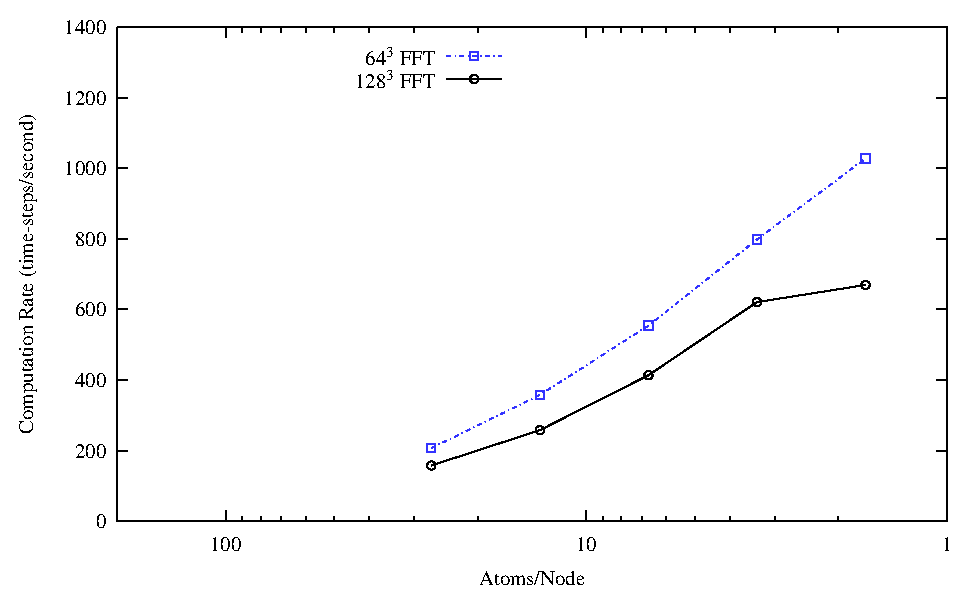
\includegraphics[keepaspectratio,width=\textwidth]{su_sope}} \\
\subfigure[Scalability data for major components of the molecular
dynamics time-step shown for two different 3D-FFT sizes, $128^3$ and $64^3$]{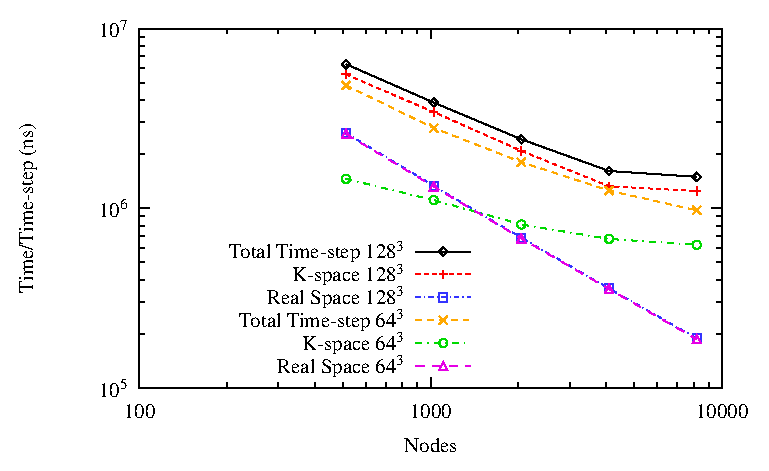
\includegraphics[keepaspectratio,width=\textwidth]{benchmark_20060726/sope_p5_breakdown_cmp}}
  \caption{The effects of changing the 3D-FFT size on the performance
    of the molecular dynamics time-step for the SOPE 13,758 atom system
    are dramatic. Note that generally use of a coarser mesh for
    the 3D-FFT decreases the accuracy of the computatation of the long
    range electrostatic forces.}
  \label{fig:sope_benchmark}
\end{figure*}


Figure ~\ref{fig:sope_benchmark} shows the elapsed time per time-step
of the SOPE molecular system. The SOPE\cite{pitman_jcp:2005} benchmark
system consists of 13,758 atoms, utilizes the Velocity Verlet
integration technique\cite{Swope1982}, and performs two 3D-FFTs
on every time-step. The results presented here were obtained using
BlueMatter software with V5 method running on the BG/L ADE
communications SPI\cite{Fitch2006}.  

  

\section{Conclusion}
\label{sec:conclusion}
This paper provides a study of the effects of several different
parallel mappings of three communication phases 
of a 3D-FFT on large number of processors. The results of our
empirical studies using the 3D-FFT show the impact of the mapping
techniques and the machine physical topology on the communication
performance of distributed memory algorithm.

Our motivation is to provide a  scalable 3D FFT on thousands of processor where the number of processors
exceeds the number independent 1D-FFTs to be computed for a given problem size, expanded checkerboard decomposition, without
any hit in the performance.   The expanded checkerboard decomposition  is used by the  Blue Matter molecular dynamics
application, which utilize one of the cores to evaluate the 3D FFT
and the other core to evaluate the real space, to scale beyond one atom per
BG/L node. The expanded checkerboard decomposition will enable applications which
utilize one of the two BG/L cores per node to compute 3D-FFT to scale
to thousands of nodes.


